\section{SelectionSort}

\subsection{Algemeen}

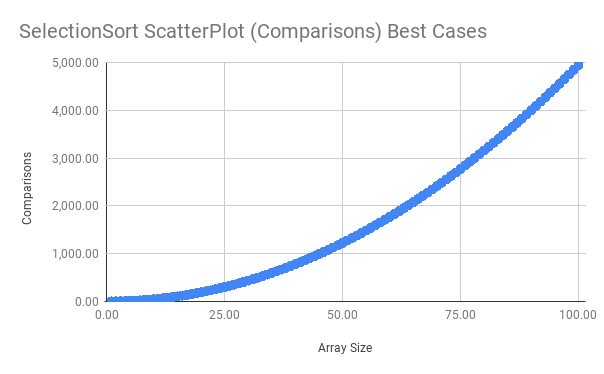
\includegraphics[scale=0.3]{sections/media/SS_C_BC}
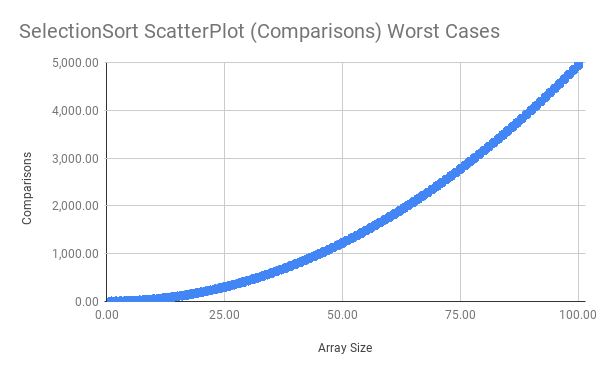
\includegraphics[scale=0.3]{sections/media/SS_C_WC}
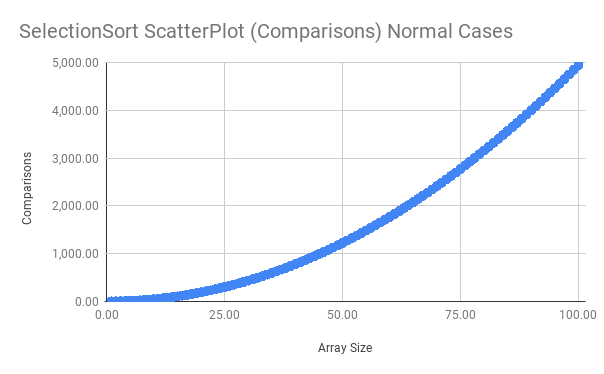
\includegraphics[scale=0.6]{sections/media/SS_C_NC}

SelectionSort is in-place vergelijkingssorteeralgoritme, het heeft een theoretische tijdscomplexiteit van \(\sim n^2/2\). Het algoritme overloopt heel de array van start tot einde, dan van start + 1 to einde, \ldots, enzovoort. Hieruit kunnen we een logisch besluit maken dat het aantal vergelijkingen gelijk zal zijn voor eenzelfde problem size.

Het eerste dat opvalt bij de data is dat de resultaten van eenzelfde problem size allemaal exact evenveel vergelijkingen gebruiken. Dit is omdat SelectionSort een constant algoritme is. Omdat het geen spreiding heeft is het een heel betrouwbaar algoritme.
